\documentclass[11pt]{article}
% \usepackage[margin=1in]{geometry}
\usepackage[top=1in, bottom=1in, left=.5in, right=.5in]{geometry} % see geometry.pdf on how to lay out the page. There's lots.
\usepackage{amsmath,amsthm,amssymb}

% Ignore spaces in filenames
\usepackage[space]{grffile}

\usepackage[T1]{fontenc}
\usepackage{bigfoot} % to allow verbatim in footnote
\usepackage[numbered,framed]{matlab-prettifier}
\usepackage{filecontents}
\usepackage{graphicx}
\usepackage[normalem]{ulem}

\let\ph\mlplaceholder % shorter macro
\lstMakeShortInline"

\lstset{
  style              = Matlab-editor,
  basicstyle         = \mlttfamily,
  escapechar         = ",
  mlshowsectionrules = true,
}

\title{MAE 275 - Midterm}
\author{John Karasinski}
\date{May 21, 2015}

\begin{document}
\maketitle

\section{Defining the System}
The state-space system can be defined,
\begin{equation}
\begin{split}
\dot{\vec{x}} = A\vec{x} + B\vec{u} \\
      \vec{y} = C\vec{x} + D\vec{u}
\end{split}
\end{equation}

\noindent where the linearized longitudinal aircraft equations of motion can be expressed in state space form, with state variables $\Delta u, \Delta w, \Delta q, \Delta \theta, \Delta h$, as
\begin{equation*}
A =
\begin{bmatrix}
    X_u & X_w & 0 & -g \cos(\theta_0) & 0 \\
    \dfrac{Z_u}{1-Z_{\dot{w}}} & \dfrac{Z_w}{1-Z_{\dot{w}}} & \dfrac{Z_q + u_0}{1-Z_{\dot{w}}} & -\dfrac{g\sin \theta_0}{1-Z_{\dot{w}}} & 0 \\
    M_u + \dfrac{M_{\dot{w}} Z_u}{1-Z_{\dot{w}}} & M_w + \dfrac{M_{\dot{w}} Z_w}{1-Z_{\dot{w}}} & M_q + \dfrac{M_{\dot{w}} (Z_q + u_0)}{1-Z_{\dot{w}}} & -\dfrac{M_{\dot{w}} g\sin \theta_0}{1-Z_{\dot{w}}} & 0 \\
    0 & 0 & 1 & 0 & 0 \\
    0 & -1 & 0 & u_0 & 0
\end{bmatrix}
\end{equation*}

\noindent Relevant B, C, and D matrices can also be formed
\begin{equation*}
B =
\begin{bmatrix}
    X_{\delta_e}                                                   & X_{\delta_T}                                                   & -X_u                                          \\
    \dfrac{Z_{\delta_e}}{1-Z_{\dot{w}}}                            & \dfrac{Z_{\delta_T}}{1-Z_{\dot{w}}}                            & \dfrac{-Z_u}{1-Z_{\dot{w}}}                   \\
    M_{\delta_e} + \dfrac{M_{\dot{w}} Z_{\delta_e}}{1-Z_{\dot{w}}} & M_{\delta_T} + \dfrac{M_{\dot{w}} Z_{\delta_T}}{1-Z_{\dot{w}}} & -M_u - \dfrac{M_{\dot{w}} Z_u}{1-Z_{\dot{w}}} \\
    0   &  0   &  0 \\
    0   &  0   &  0 \\
\end{bmatrix}
\end{equation*}

\begin{equation*}
C =
\begin{bmatrix}
    1 &          0     & 0 & 0   & 0\\
    0 & \dfrac{1}{u_0} & 0 & 0   & 0\\
    0 &          0     & 0 & 0   & 1\\
    0 &         -1     & 0 & u_0 & 0\\
    0 &          0     & 0 & 1   & 0\\
\end{bmatrix}
\end{equation*}

\begin{equation*}
D =
\begin{bmatrix}
    0 & 0 & 0 \\
    0 & 0 & 0 \\
    0 & 0 & 0 \\
    0 & 0 & 0 \\
    0 & 0 & 0 \\
\end{bmatrix}
\end{equation*}

\clearpage
\noindent Using the longitudinal equations of motion for C-5A for level flight ($u_0=246$ ft/s) at sea level, the resultant system is
$$
\vec{x}= \left[ \begin{array}{c}        u \\ w        \\ q   \\ \theta \\       h \end{array} \right], \qquad
\vec{u}= \left[ \begin{array}{c} \delta_e \\ \delta_T \\ u_g                      \end{array} \right], \qquad
\vec{y}= \left[ \begin{array}{c}        u \\ \alpha   \\ h   \\ \dot{h} \\ \theta \end{array} \right] 
$$

$$
\dot{\vec{x}} = \left[ \begin{array}{ccccc}
  -0.0214              &  +0.0957             &    0      &  -32.2 & 0 \\
   -0.231              &  -0.634              & +246      &    0   & 0 \\
   +1.964\times10^{-4} &  -8.895\times10^{-4} &   -0.8275 &    0   & 0 \\
    0                  &   0                  &    1      &    0   & 0 \\
    0                  &  -1                  &    0      & +246   & 0 \end{array} \right]
\vec{x} + \left[\begin{array}{ccc}
      +0.45            & +0.554\times10^{-4}  & +0.0214                \\ 
      -9.53            & -0.193\times10^{-5}  & +0.231                 \\
    -0.6795            & +1.4571\times10^{-7} & -1.9642\times10^{-4}   \\ 
          0            &  0                   &  0                     \\ 
          0            &  0                   &  0 \end{array}\right] \vec{u}  
$$

$$
\vec{y} = \left[ \begin{array}{ccccc}
         1 &   0      &   0   &    0   &  0 \\
         0 &   0.0041 &   0   &    0   &  0 \\
         0 &   0      &   0   &    0   &  1 \\
         0 &  -1      &   0   &  246   &  0 \\
         0 &   0      &   0   &    1   &  0 \end{array} \right]
\vec{x}+\left[\begin{array}{ccc}
         0 &   0      & 0 \\ 
         0 &   0      & 0 \\
         0 &   0      & 0 \\
         0 &   0      & 0 \\
         0 &   0      & 0 \end{array}\right]\vec{u}
$$
         
\vspace{25pt}
The loops are sequentially closed in the order: $\theta\rightarrow\delta_e$, $u\rightarrow\delta_T$, $\dot{h}\rightarrow\theta_e$.
The following page lists the linearized transfer functions used to design the compensators, along with the transfer function of each compensator.
The gain and phase margins and bandwidth are also listed for the compensated loop.

% \noindent with $x = [\Delta v, \Delta p, \Delta r, \Delta \varphi, \Delta \psi]$ and $u =[\Delta \delta_r, \Delta \delta_a]$. Plugging in the data for the DC-8 aircraft in Flight Condition 8002 from Appendix A of "Aircraft Dynamics and Automatic Control" yields
% \begin{equation*}
% A =
% \begin{bmatrix}
%   -1.0080e-1 &          0 & -4.6820e+2 & +3.2200e+1  &          0 \\
%   -5.7881e-3 & -1.2320e+0 & +3.9700e-1 &          0  &          0 \\
%   +2.7787e-3 & -3.4600e-2 & -2.5700e-1 &          0  &          0 \\
%            0 &          1 &          0 &          0  &          0 \\
%            0 &          0 &          1 &          0  &          0 \\

% \end{bmatrix}
% \end{equation*}

% \begin{equation*}
% B =
% \begin{bmatrix}
%   +1.3480e+1 &          0 \\
%   +3.9200e-1 & -1.6200e+0 \\
%   -8.6400e-1 & -1.8750e-2 \\
%            0 &          0 \\
%            0 &          0 \\
% \end{bmatrix}
% \end{equation*}

% \begin{equation*}
% C =
% \begin{bmatrix}
%    +2.1358e-3 &           0 &           0  &          0 &           0 \\
%             0 &           0 &           1  &          0 &           0 \\
%             0 &           0 &           0  &          1 &           0 \\
% \end{bmatrix}
% \end{equation*}

% \begin{equation*}
% D =
% \begin{bmatrix}
%      0  &   0 \\
%      0  &   0 \\
%      0  &   0 \\
% \end{bmatrix}
% \end{equation*}

% \clearpage
% \section{Designing the Controllers}
% Two controllers were designed. The first controller, $Gc_{\phi}$ was designed as
% \begin{filecontents*}{code.m}
%   -360.94 (s+1.413) (s+0.07616)
%   -----------------------------
%          s (s+100) (s+3)
% \end{filecontents*}
% \lstinputlisting[]{code.m}

% \noindent This controller was determined using loop-shaping principles such that it had a roll-attitude bandwidth of $\sim$3 rad/sec (-3dB criterion) and a minimum overshoot in step response. \\

% \begin{figure}[h!]
% \begin{center}
% 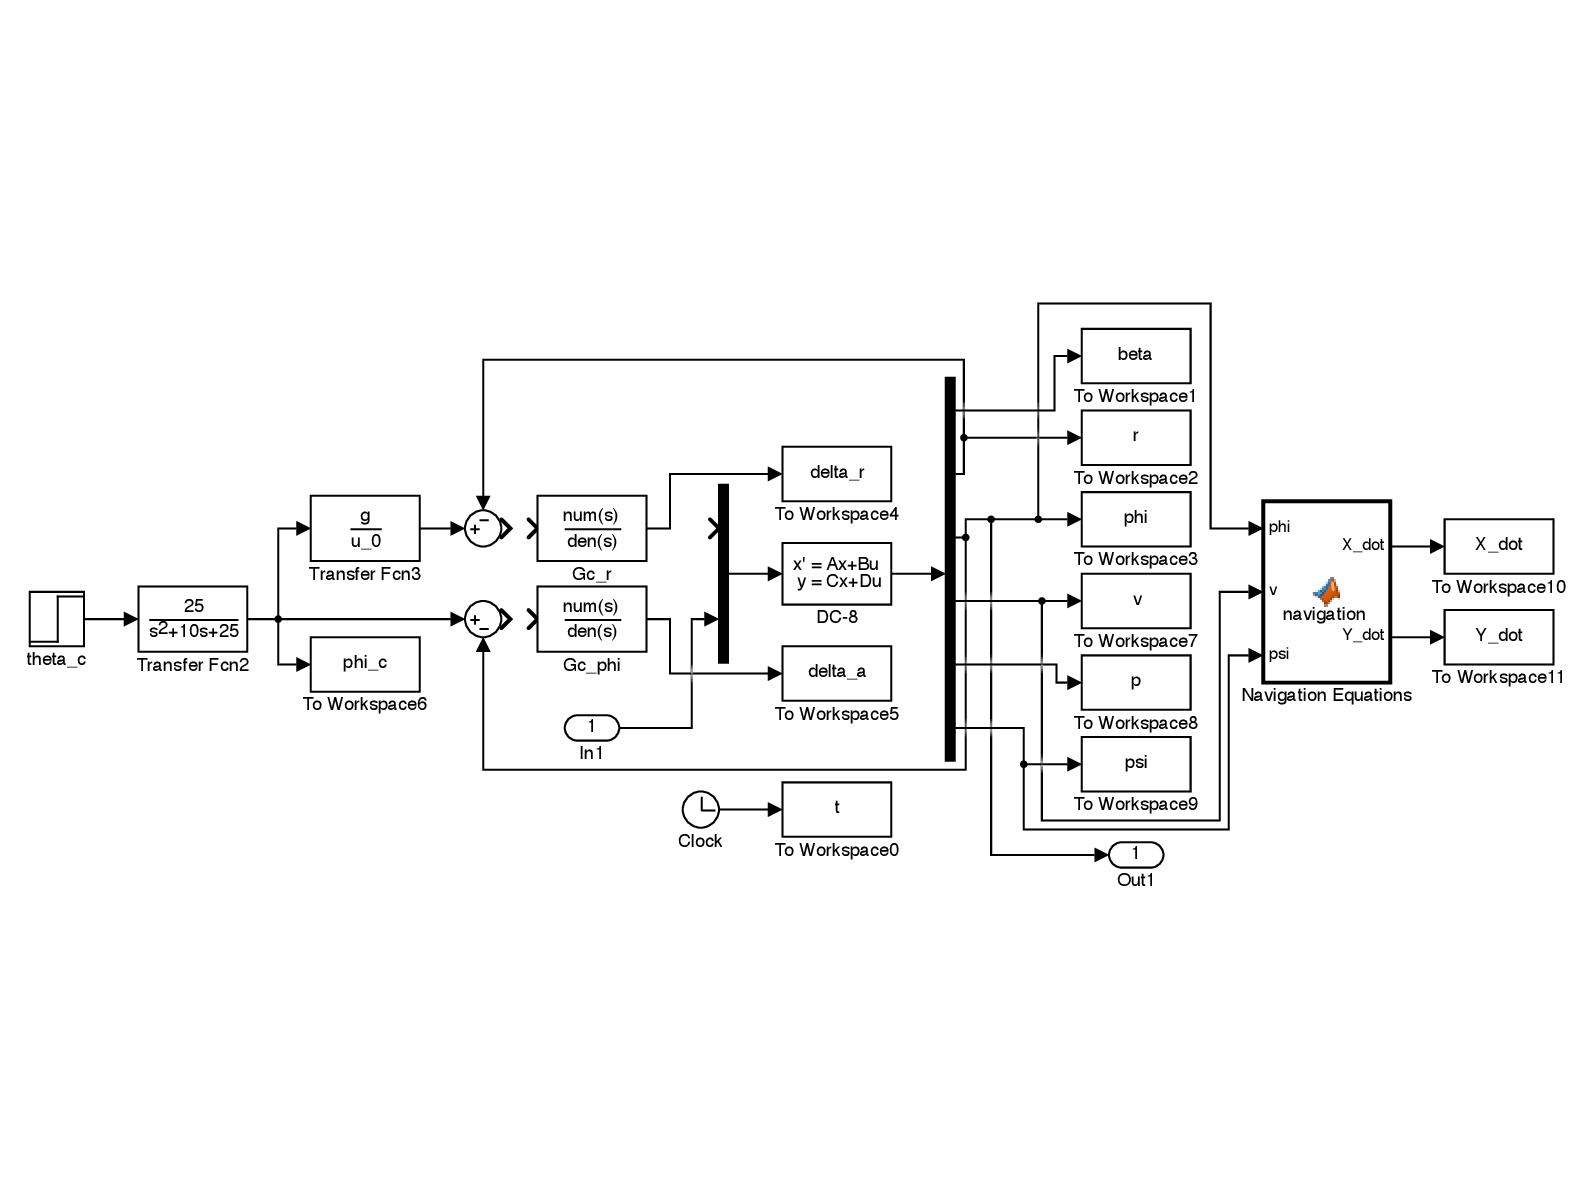
\includegraphics[height=.425\textheight]{figures/first_controller_simulink}
% \caption{Simulink Diagram for First Controller Design}
% \end{center}
% \end{figure}

% \begin{figure}[h!]
% \begin{center}
% 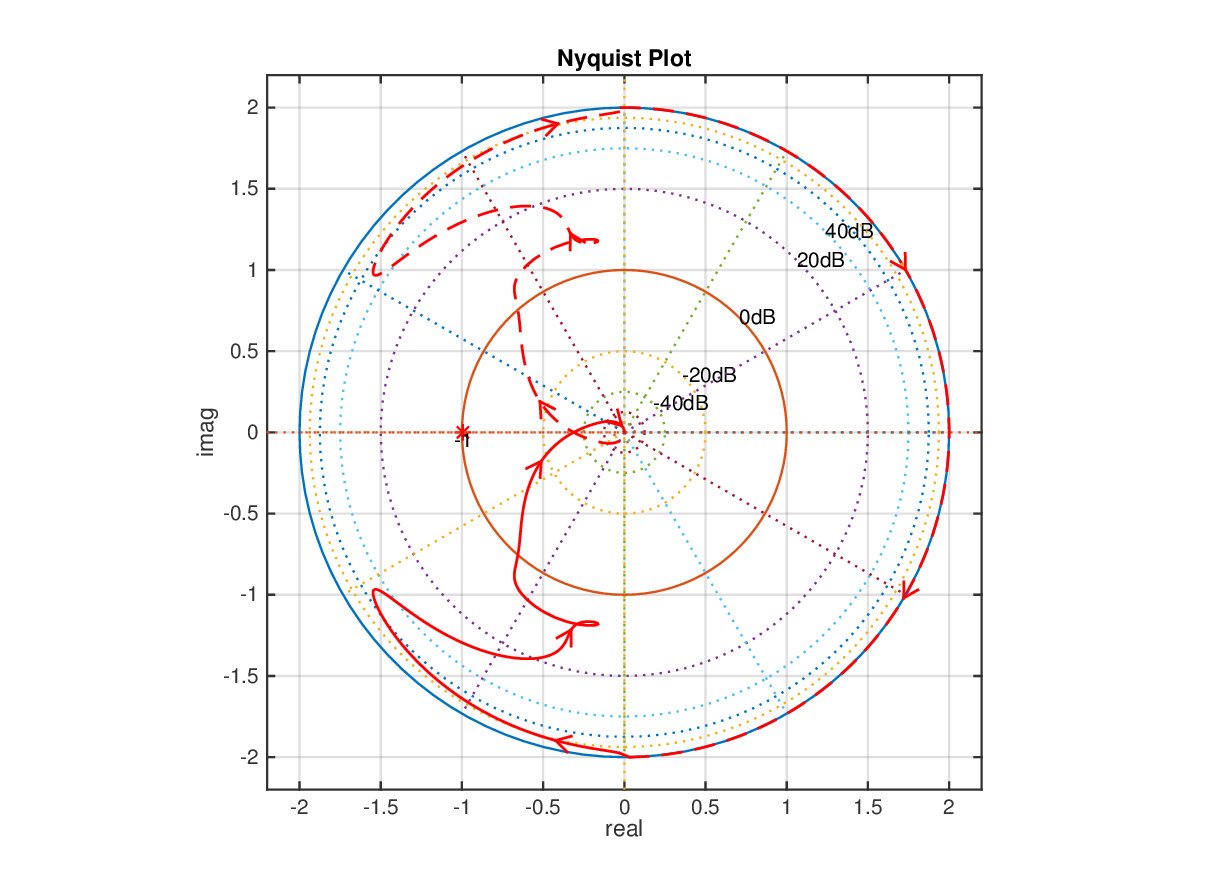
\includegraphics[height=.425\textheight]{figures/phi_nyquist2}
% \caption{Nyquist Diagram for First Controller Design}
% \end{center}
% \end{figure}

% \noindent The second controller, $Gc_r$ was designed as
% \begin{filecontents*}{code.m}
%   21.969 (s-1.86)
%   ----------------
%   (s+10) (s+8.199)
% \end{filecontents*}
% \lstinputlisting[]{code.m}

% \noindent This controller was determined using loop-shaping principles such that it had a bandwidth of $\sim$1 rad/sec (-3dB criterion), giving a factor of approximately three between r-loop and $\phi$-loop bandwidths. \\

% \begin{figure}[h!]
% \begin{center}
% 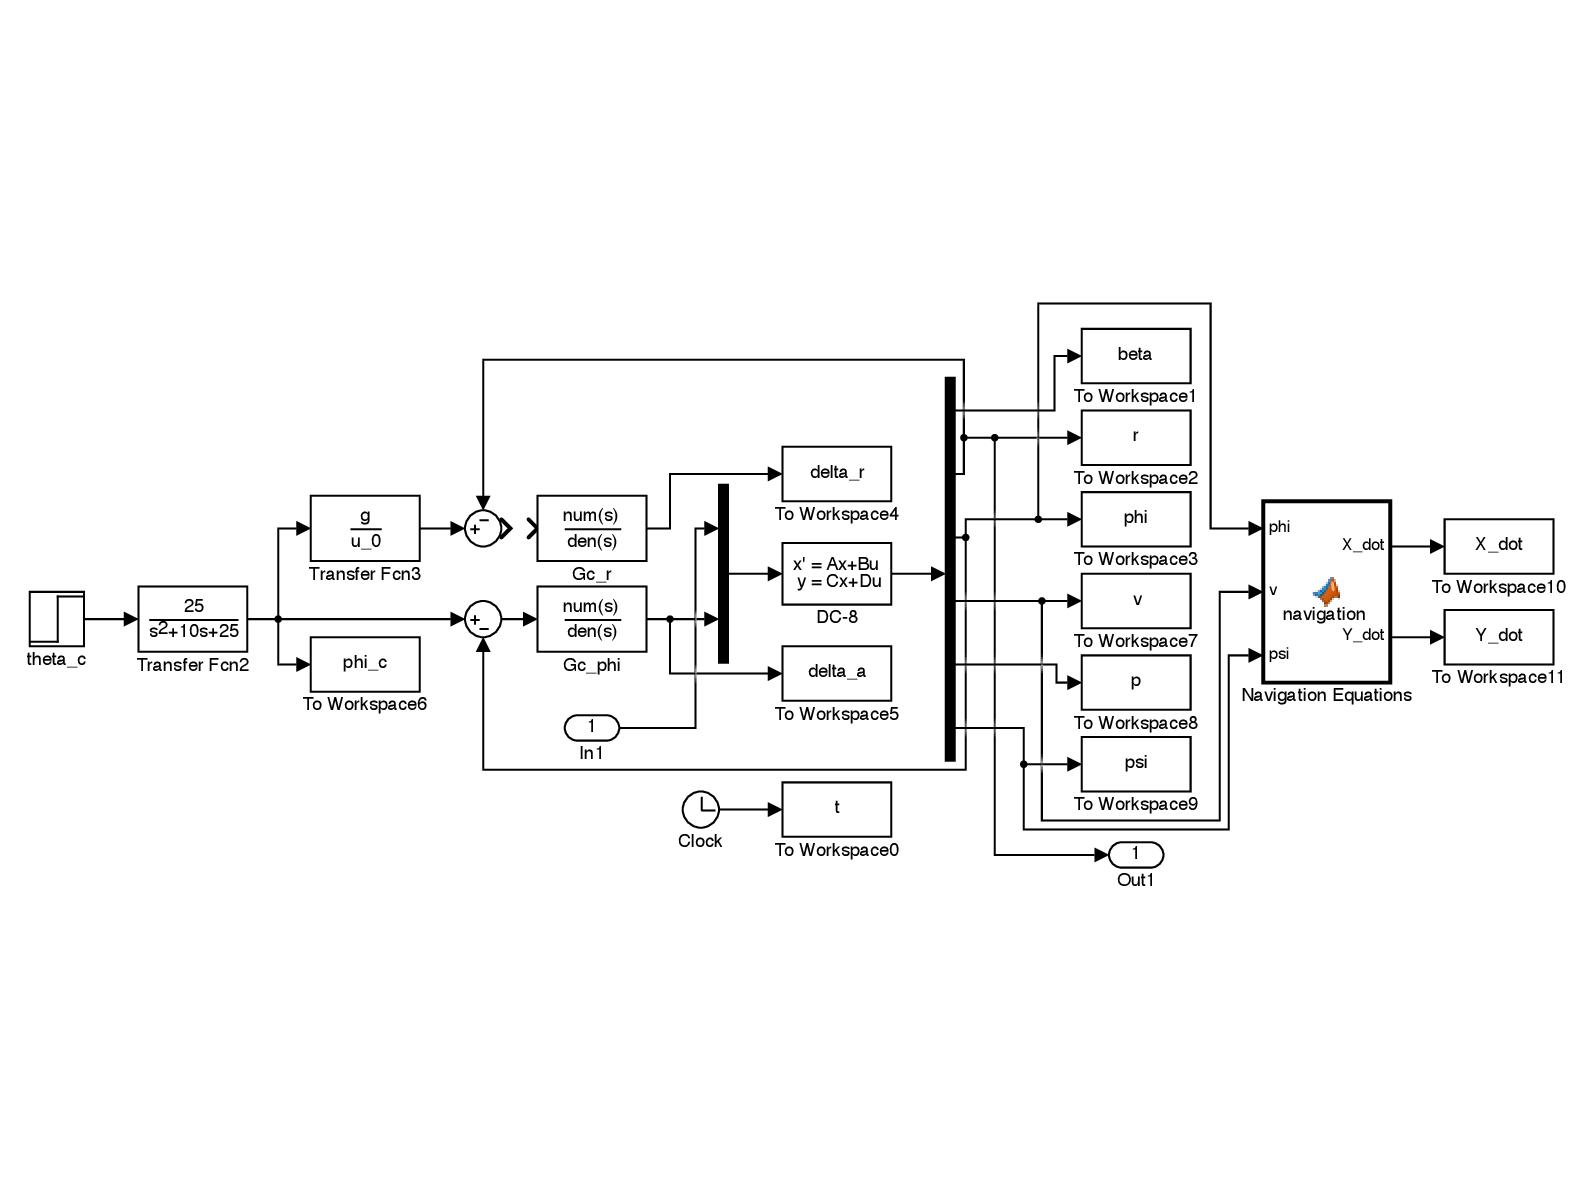
\includegraphics[height=.425\textheight]{figures/second_controller_simulink}
% \caption{Simulink Diagram for Second Controller Design}
% \end{center}
% \end{figure}

% \begin{figure}[h!]
% \begin{center}
% 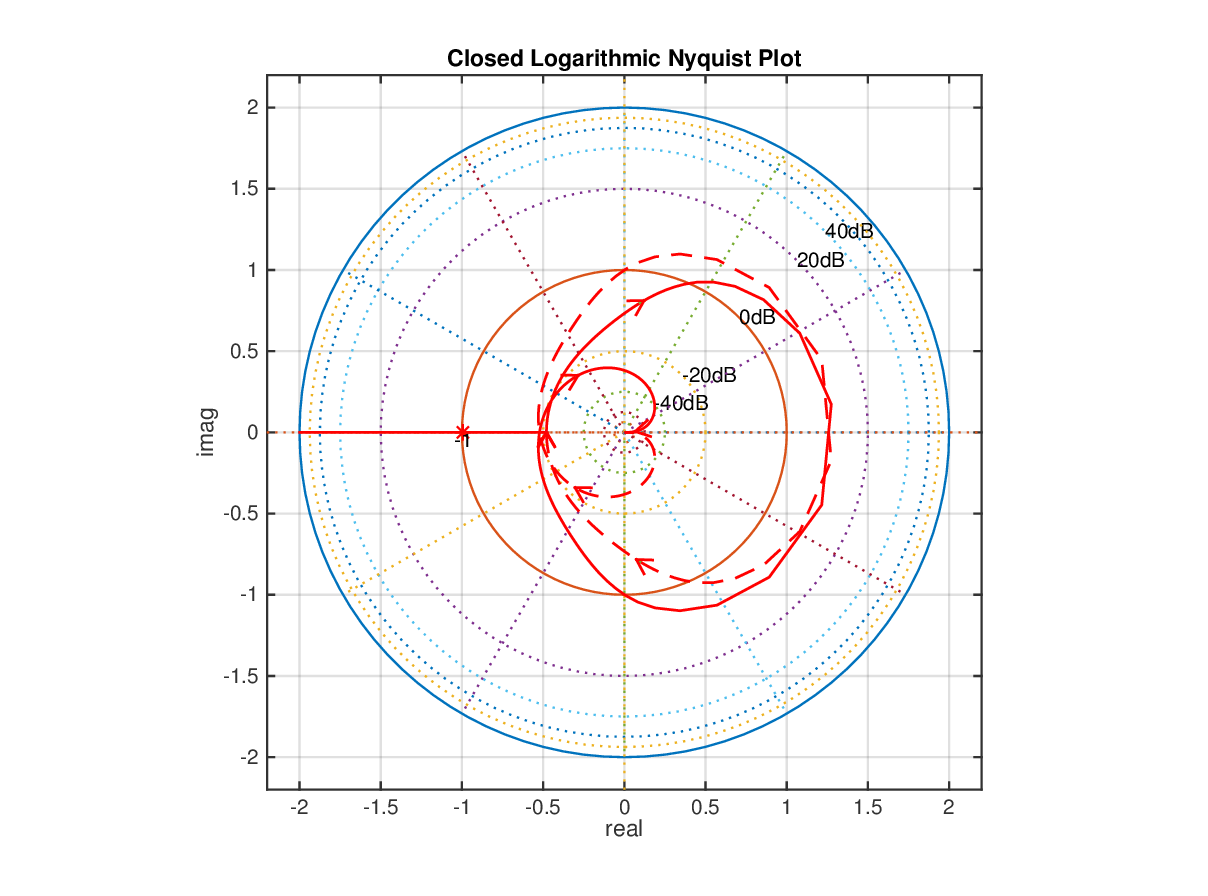
\includegraphics[height=.425\textheight]{figures/r_nyquist2}
% \caption{Nyquist Diagram for Second Controller Design}
% \end{center}
% \end{figure}

% \noindent Additionally, both controllers have:

% more poles than zeros (are strictly proper compensators)

% gain margins of at least 12dB

% phase margins of at least 40 deg

% \clearpage
% \begin{figure}[h!]
% \begin{center}
% 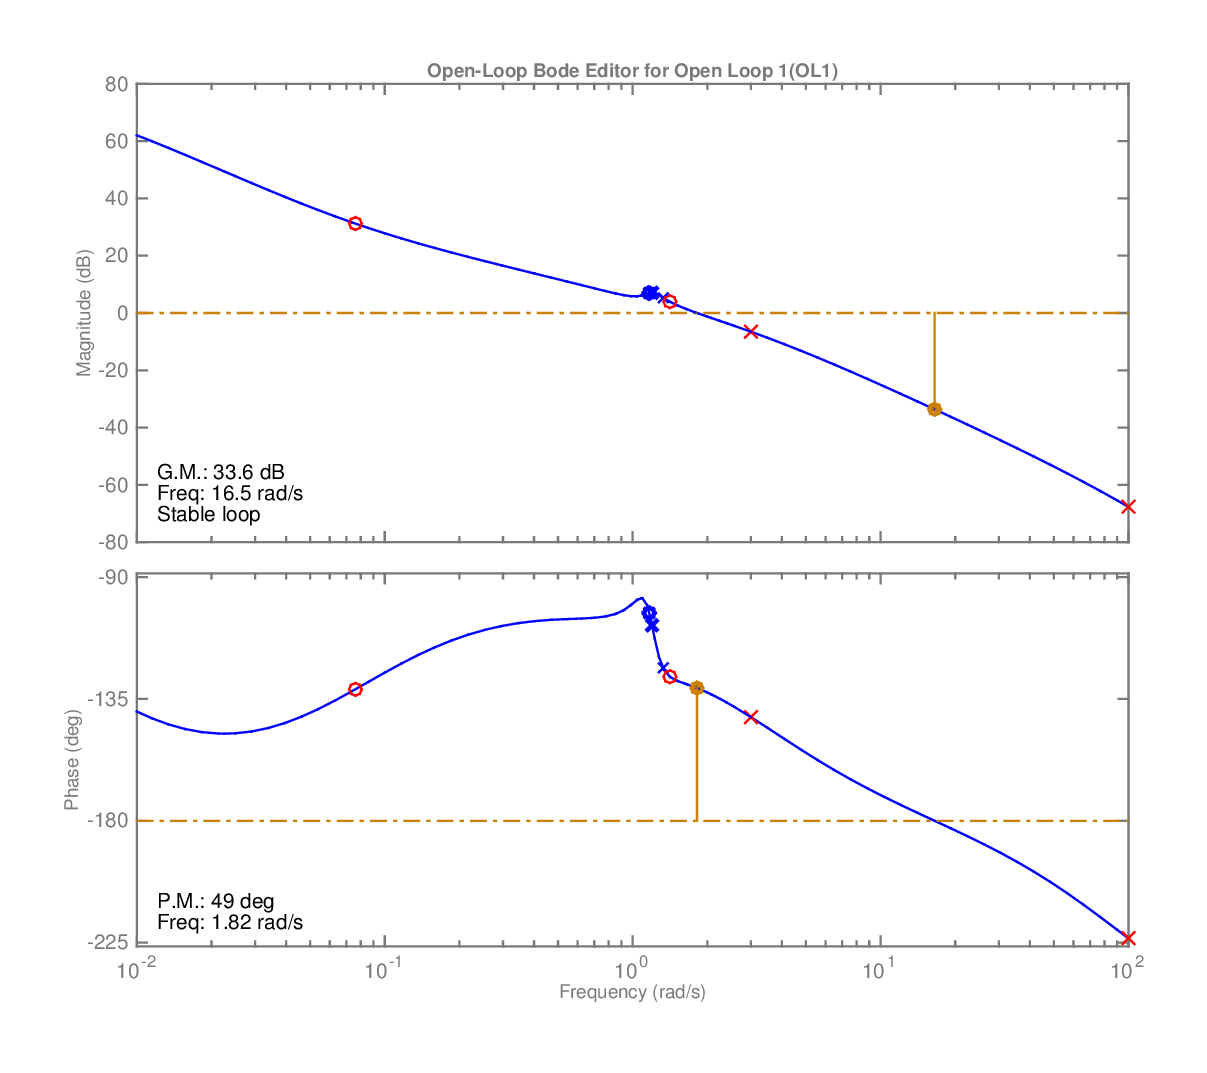
\includegraphics[height=.435\textheight]{figures/phi_delta_a_open_loop}
% \caption{$\phi$-loop open-loop Bode with G.M. of 34 dB and P.M. of 49 deg}
% \end{center}
% \end{figure}

% \begin{figure}[h!]
% \begin{center}
% 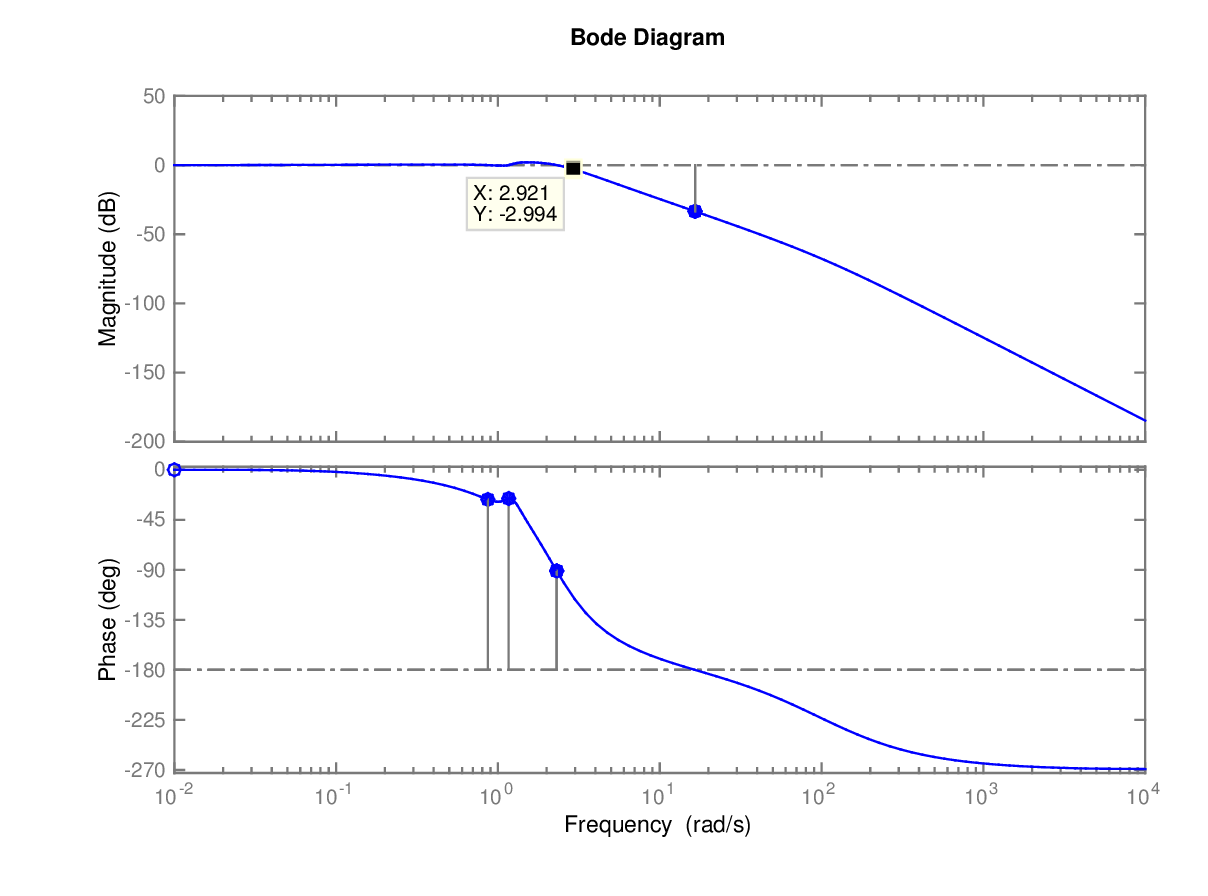
\includegraphics[height=.375\textheight]{figures/phi_delta_a_closed_loop}
% \caption{$\phi$-loop closed-loop Bode with bandwidth of 3 rad/s (3dB criterion)}
% \end{center}
% \end{figure}

% \begin{figure}[h!]
% \begin{center}
% 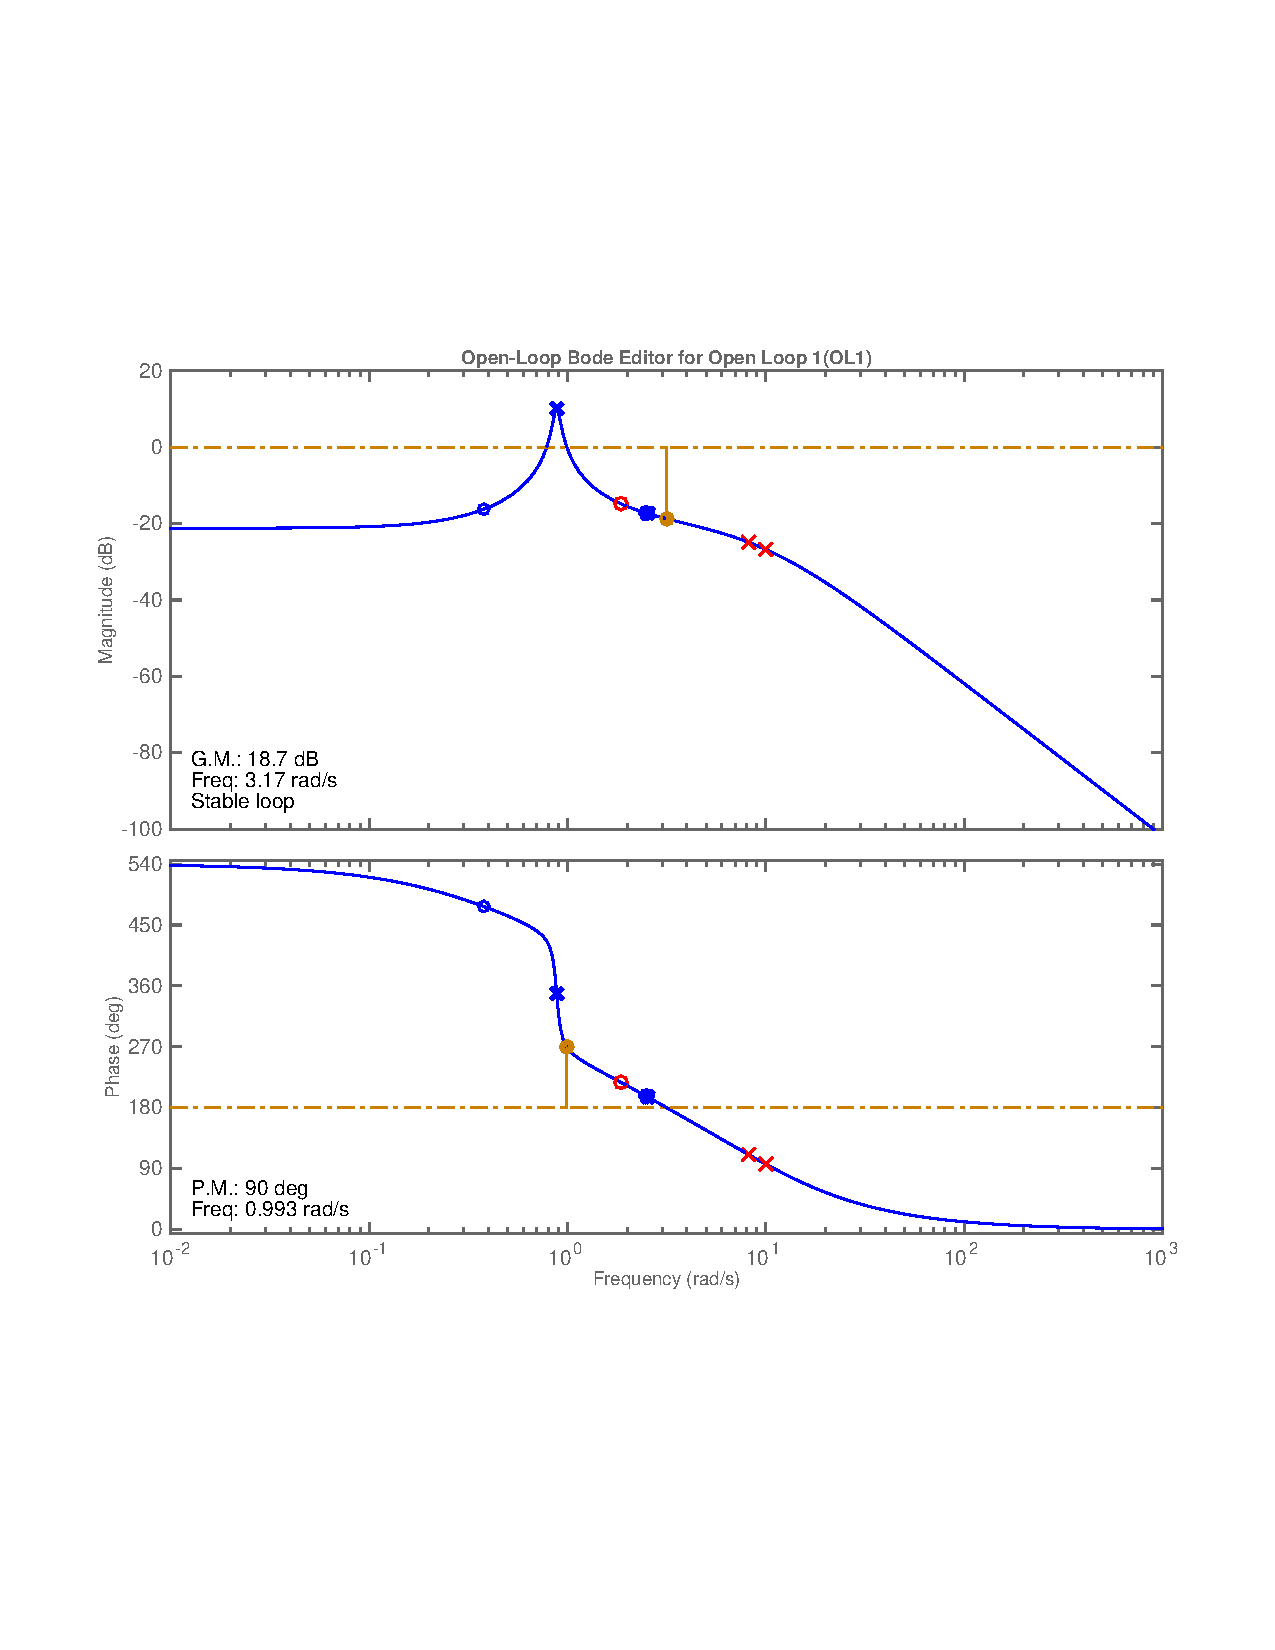
\includegraphics[height=.435\textheight]{figures/r_delta_r_open_loop}
% \caption{$r$-loop open-loop Bode with G.M. of 18 dB and P.M. of 90 deg}
% \end{center}
% \end{figure}

% \begin{figure}[h!]
% \begin{center}
% 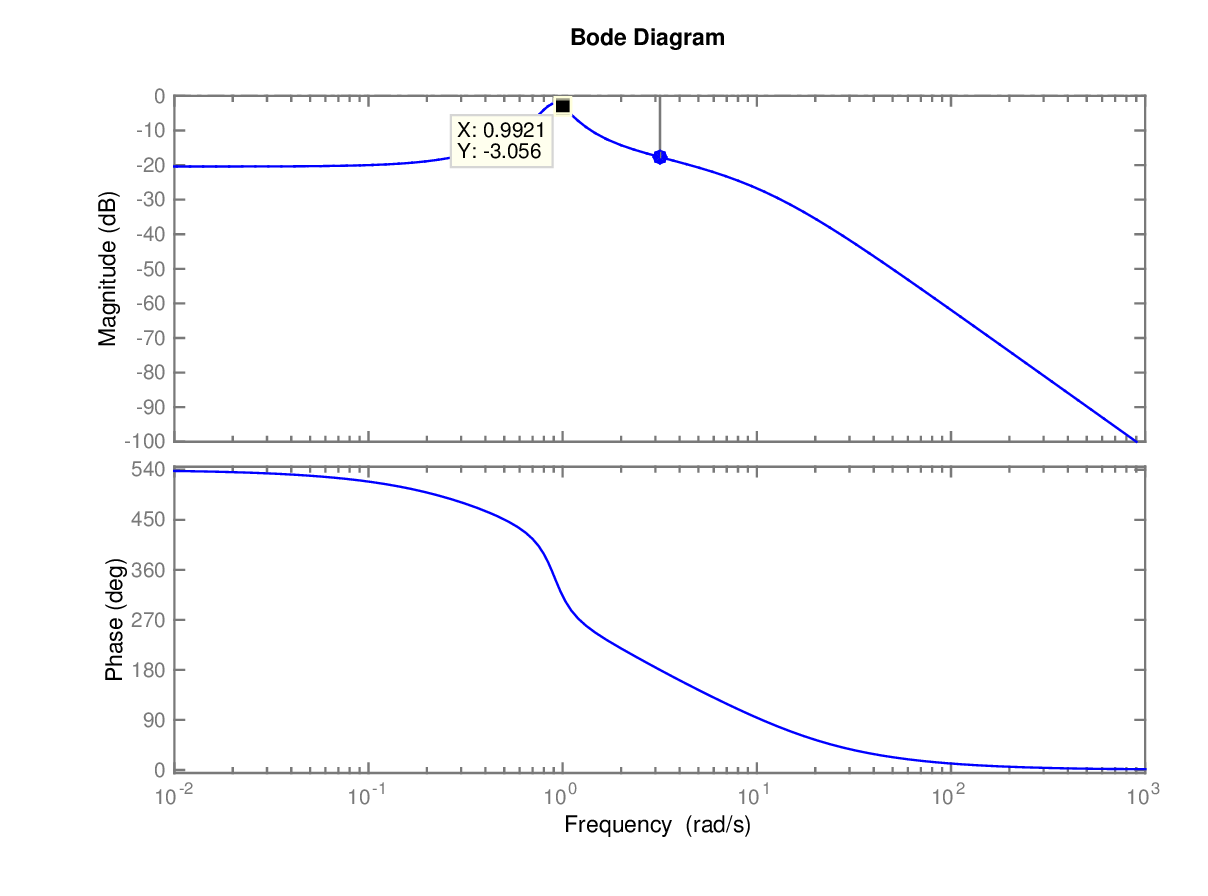
\includegraphics[height=.375\textheight]{figures/r_delta_r_closed_loop}
% \caption{r-loop closed-loop Bode with bandwidth of 1 rad/s (3dB criterion)}
% \end{center}
% \end{figure}

% \clearpage
% \section{Final Simulink Diagram}
% \begin{figure}[h!]
% \begin{center}
% 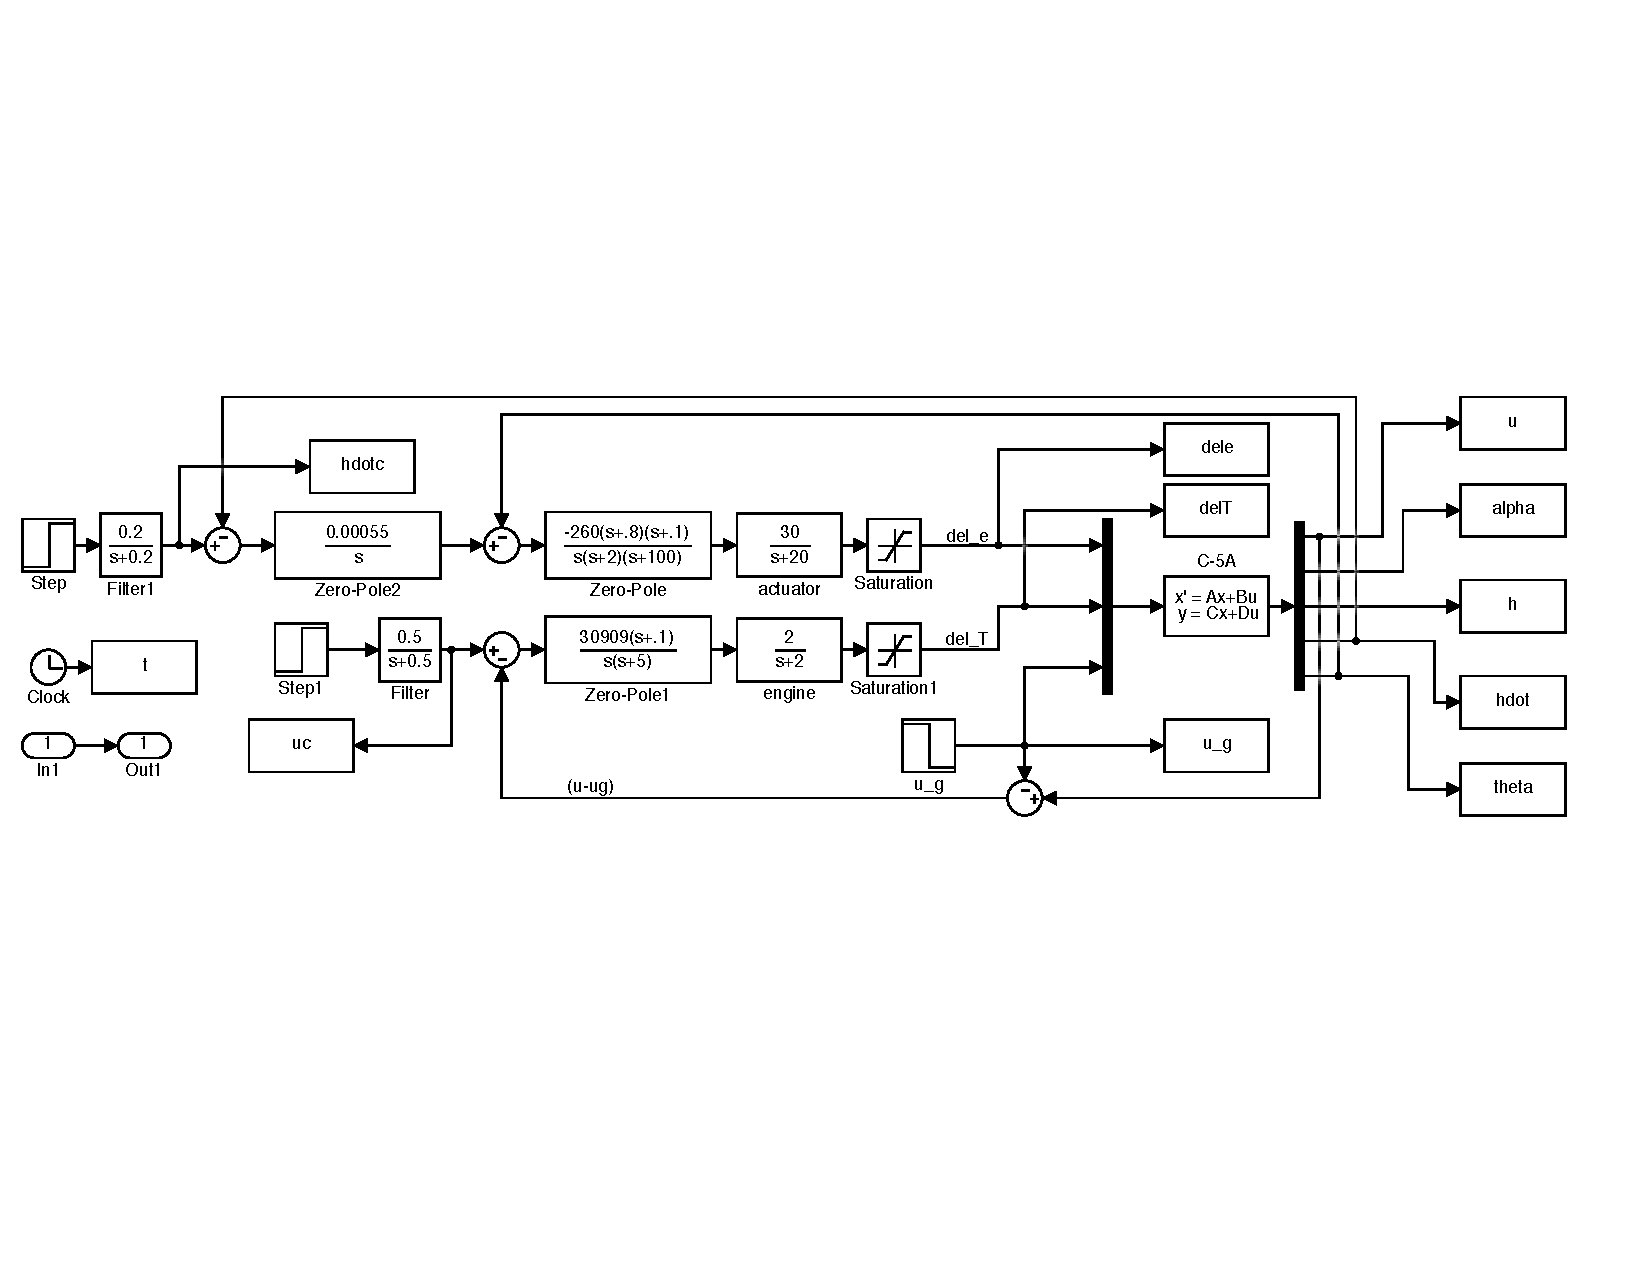
\includegraphics[width=1\textwidth]{figures/final_simulink}
% \caption{Final Simulink Diagram}
% \end{center}
% \end{figure}

% \noindent Where the navigation function is defined as
% \begin{filecontents*}{code.m}
% function [X_dot, Y_dot] = navigation(phi, v, psi)
% %#codegen

% theta = 0;
% U = 468.2;
% V = v;
% W = 0;

% X_dot = U * (cos(psi) * cos(theta)) + ...
%         V * (cos(psi) * sin(theta) * sin(phi) - sin(psi) * cos(phi)) + ...
%         W * (cos(psi) * sin(theta) * cos(phi) + sin(psi) * sin(phi));

% Y_dot = U * (sin(psi) * cos(theta)) + ...
%         V * (sin(psi) * sin(theta) * sin(phi) - cos(psi) * cos(phi)) + ...
%         W * (sin(psi) * sin(theta) * cos(phi) + cos(psi) * sin(phi));
% \end{filecontents*}
% \lstinputlisting[]{code.m}

% \clearpage
% \section{Results}

% \begin{figure}[h!]
% \begin{center}
% 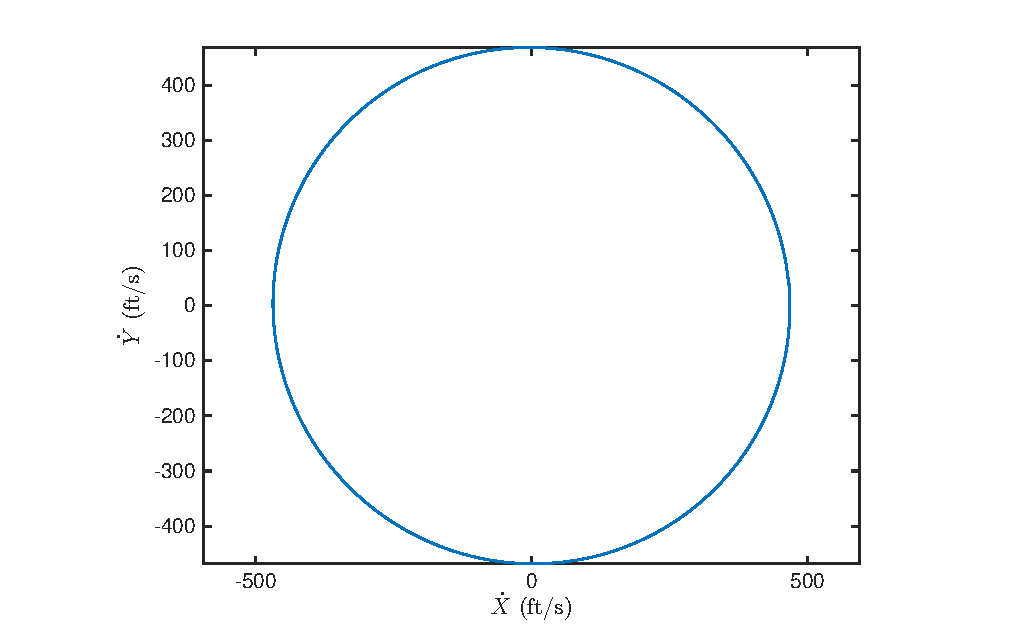
\includegraphics[width=.85\textwidth]{figures/circle}
% \caption{Demonstration of turn-coordination from $\sim$ 267 second simulation}
% \end{center}
% \end{figure}

% \begin{figure}[h!]
% \begin{center}
% 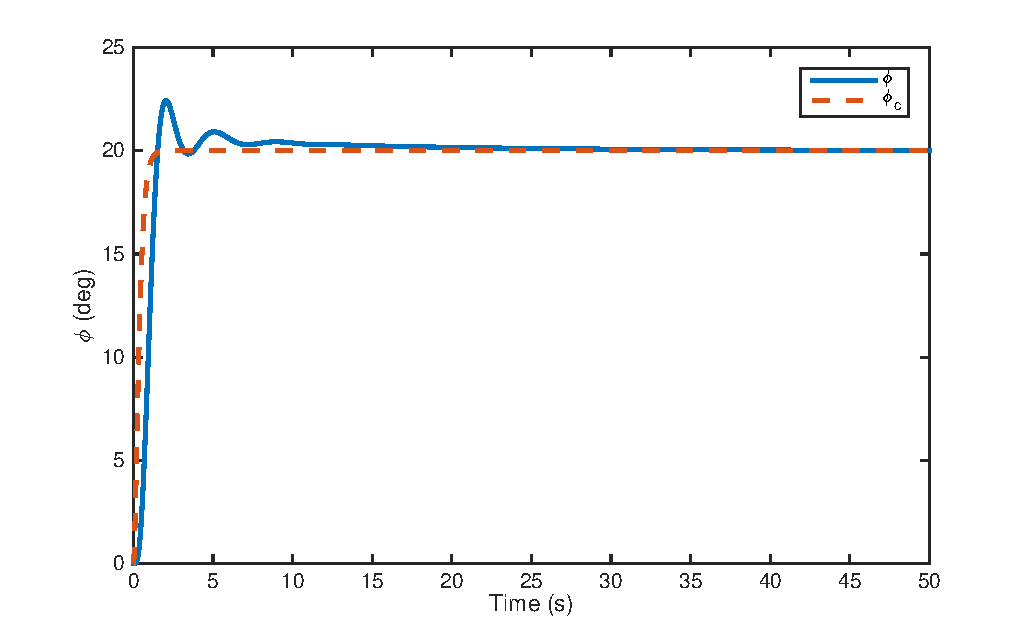
\includegraphics[width=.85\textwidth]{figures/phi}
% \caption{$\phi$ response to $\phi_c$, showing $\sim 10\%$ overshoot}
% \end{center}
% \end{figure}

% \clearpage
% \begin{figure}[h!]
% \begin{center}
% 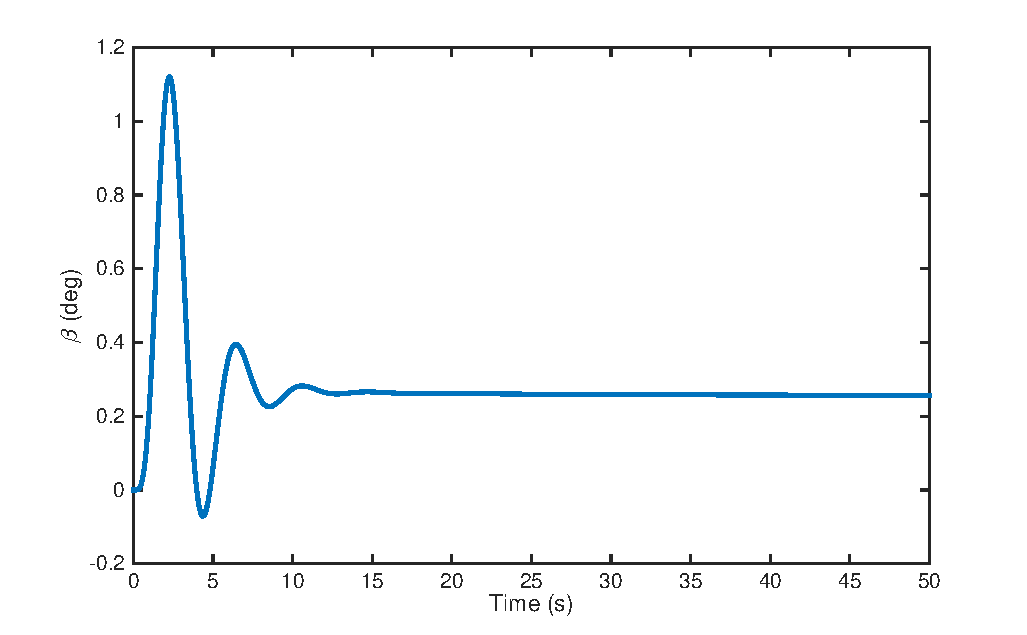
\includegraphics[height=.4\textheight]{figures/beta}
% \caption{$\beta$ Response}
% \end{center}
% \end{figure}

% \begin{figure}[h!]
% \begin{center}
% 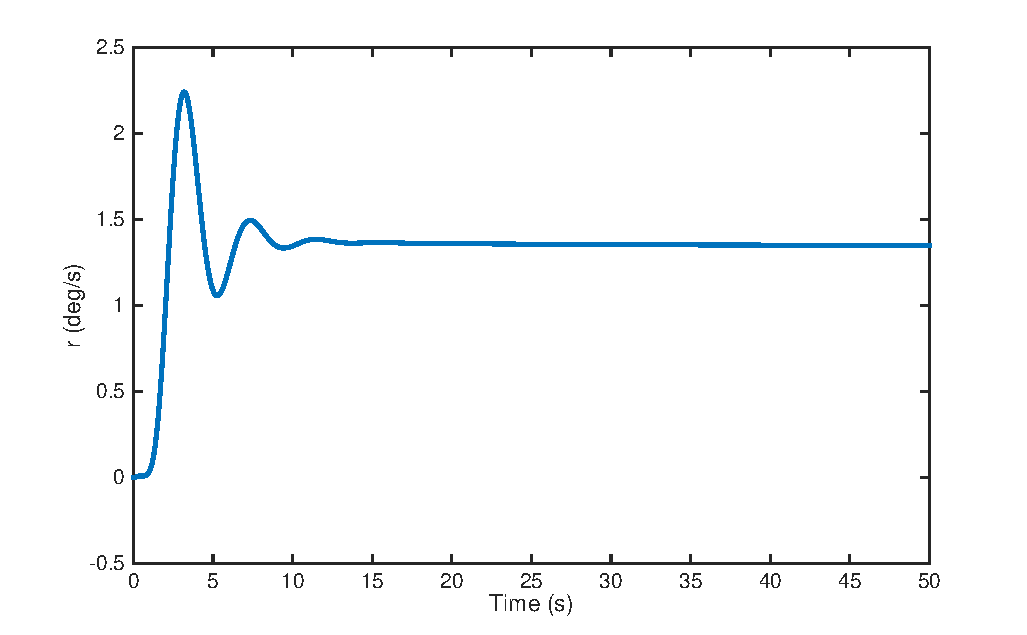
\includegraphics[height=.4\textheight]{figures/r}
% \caption{$r$ Response}
% \end{center}
% \end{figure}

% \clearpage
% \begin{figure}[h!]
% \begin{center}
% 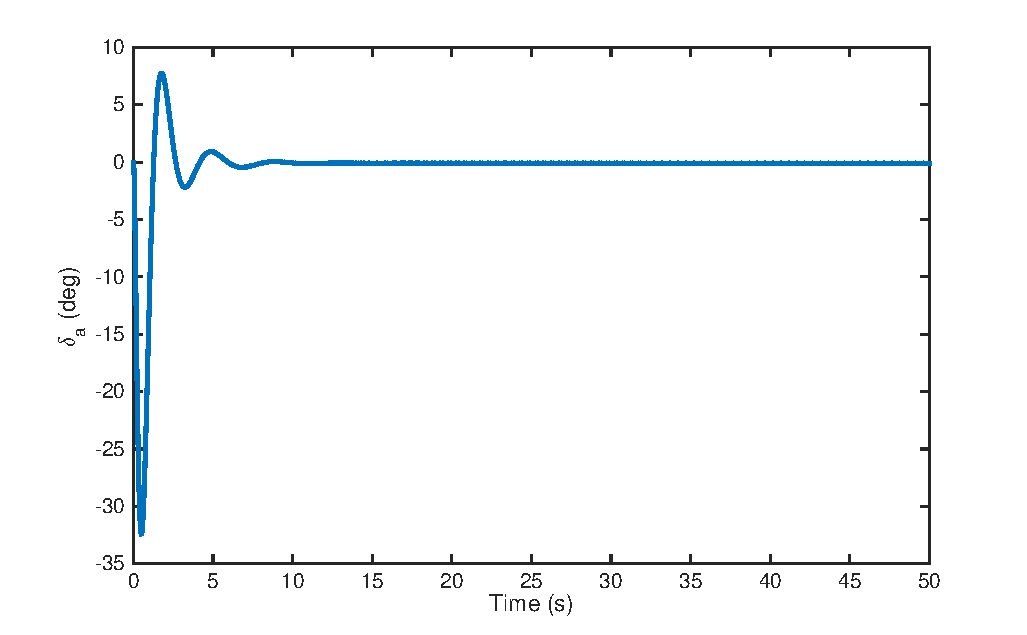
\includegraphics[height=.4\textheight]{figures/delta_a}
% \caption{$\delta_a$ Input}
% \end{center}
% \end{figure}

% \begin{figure}[h!]
% \begin{center}
% 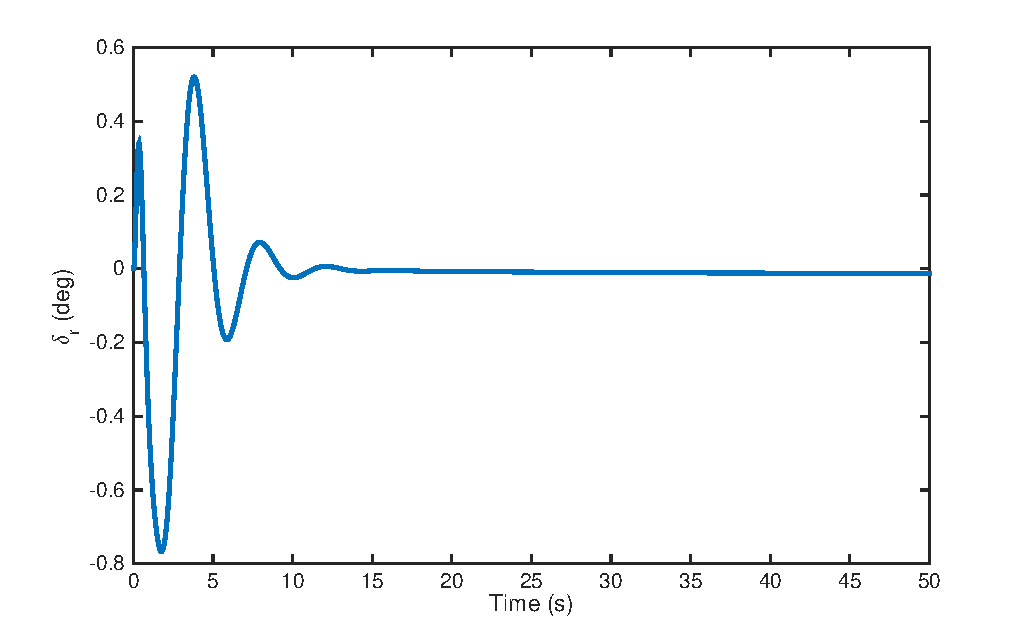
\includegraphics[height=.4\textheight]{figures/delta_r}
% \caption{$\delta_r$ Input}
% \end{center}
% \end{figure}

% \section{Handling Qualities}
% The handling qualities of the aircraft with the designed controllers can be estimated using the Bandwidth/Phase-Delay boundaries explained in the handout. The bandwidth is defined as $w_{BW_{phase}} = 3.82$ rad/s. The phase delay, $\tau_p$ is defined
% \begin{equation*}
% \tau_p = \dfrac{\Delta \Phi 2w_{180}}{57.3 (2w_{180})} = \dfrac{(-179.7) - (-193.3)}{57.3 (2*32.54)} = 0.003 \mbox{s}
% \end{equation*}
% These values suggest Level 1 handling qualities.
% \begin{figure}[h!]
% \begin{center}
% 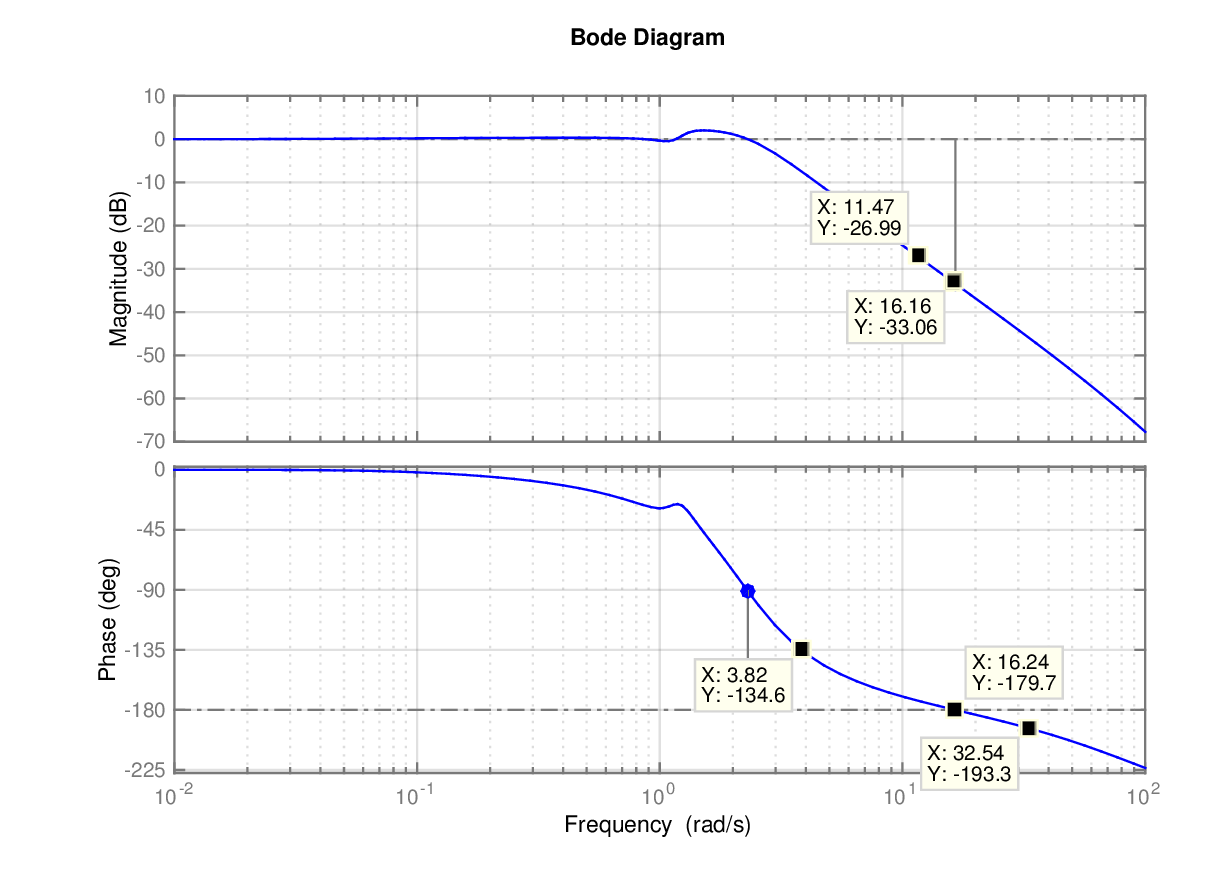
\includegraphics[height=.4\textheight]{figures/all}
% \caption{Closed-loop Bode with relevant points selected}
% \end{center}
% \end{figure}

% \begin{figure}[h!]
% \begin{center}
% 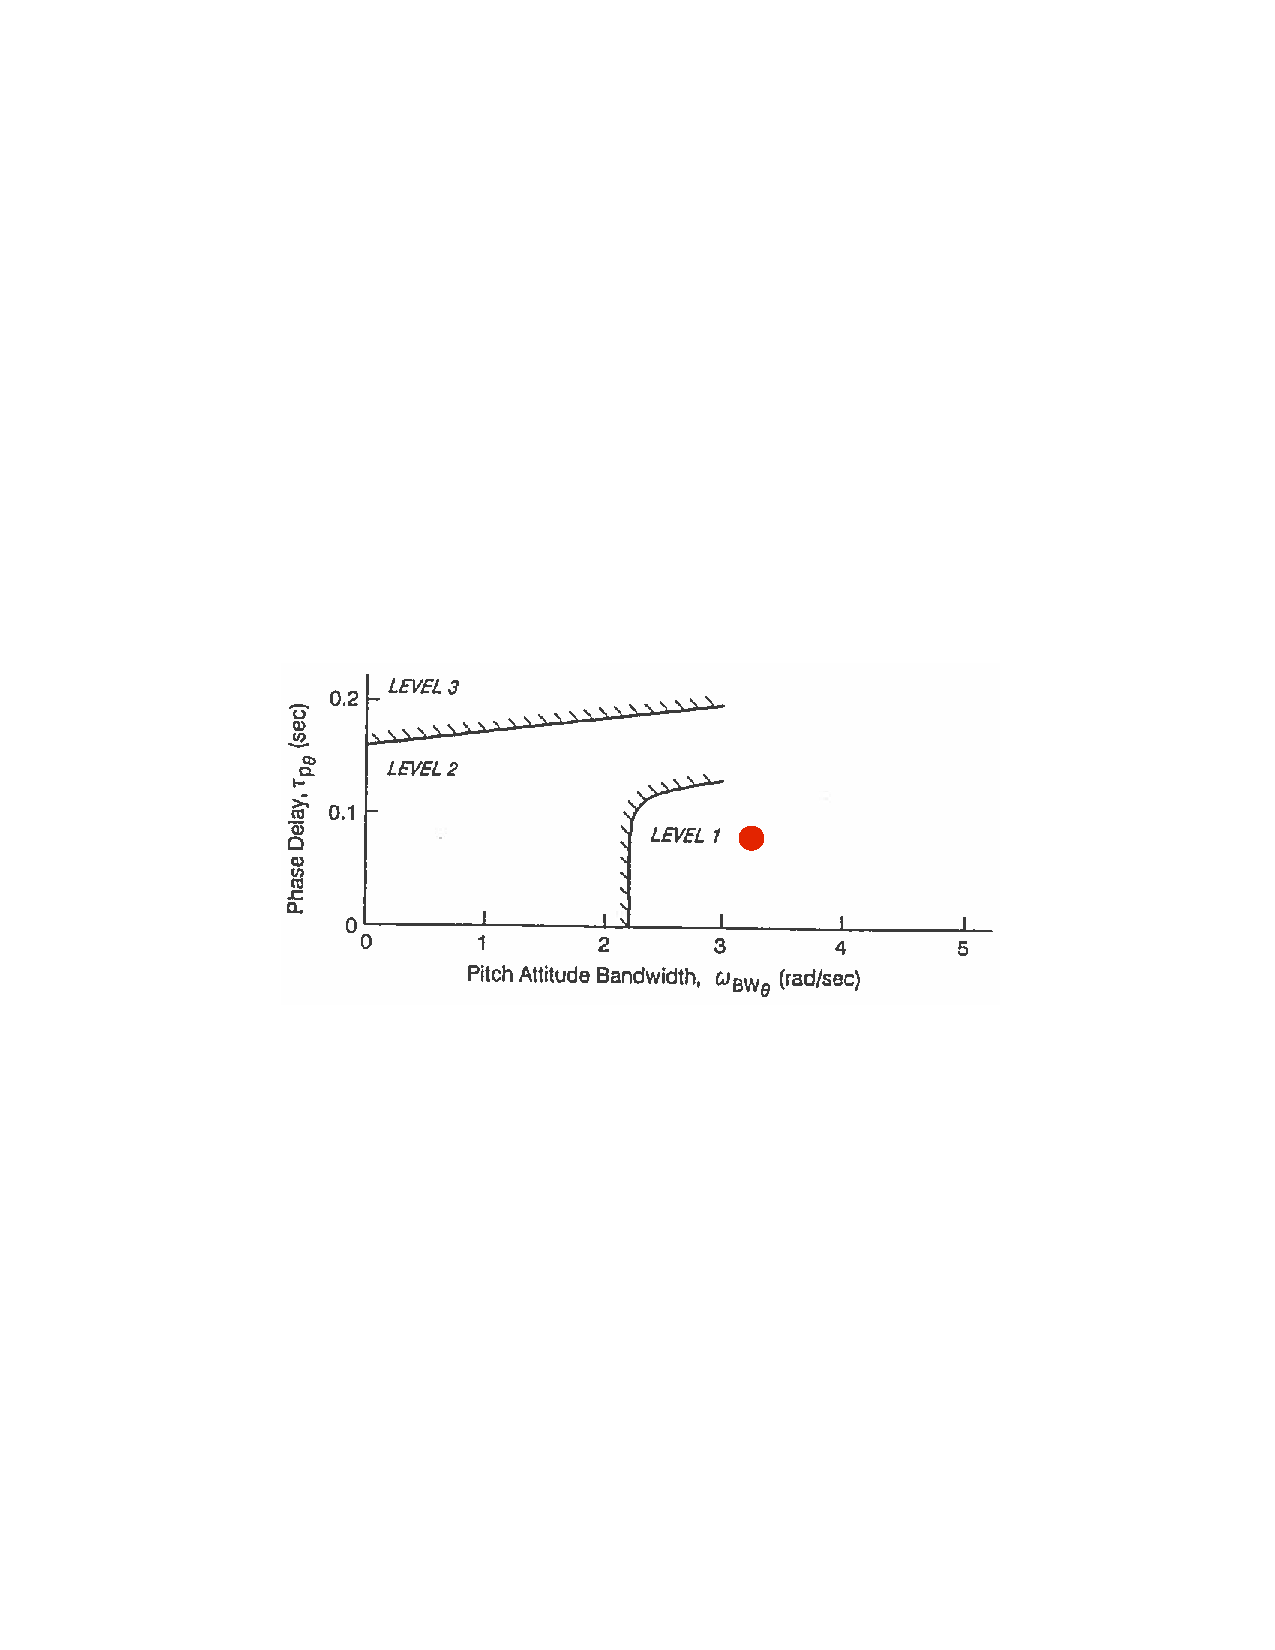
\includegraphics[height=.2\textheight]{figures/handling_marked}
% \caption{Handling qualities plot with location marked}
% \end{center}
% \end{figure}

\end{document}
